\documentclass[14pt,a4paper,xcolor=svgnames]{beamer}
\setbeamertemplate{navigation symbols}{}
% \usepackage[svgnames]{xcolor}
 \usepackage{setspace}
% \onehalfspacing

\usepackage{tikz}
\usetikzlibrary{mindmap,trees,backgrounds}

\begin{document}
% \pagestyle{empty}
\tikzset{every concept/.append style={font=\LARGE, minimum size=4cm, outer sep=-1pt, inner sep=5pt, text width=6.5cm}}
\tikzset{level 1 concept/.append style={level distance=15cm, sibling angle=70}}
\tikzset{level 2 concept/.append style={level distance=10cm}}
\tikzset{every annotation/.style={text=white,inner sep=2mm,text centered, font=\rm}}

\begin{frame}[plain]
\setstretch{1.45}
\begin{center}
\resizebox{\textwidth}{!}{
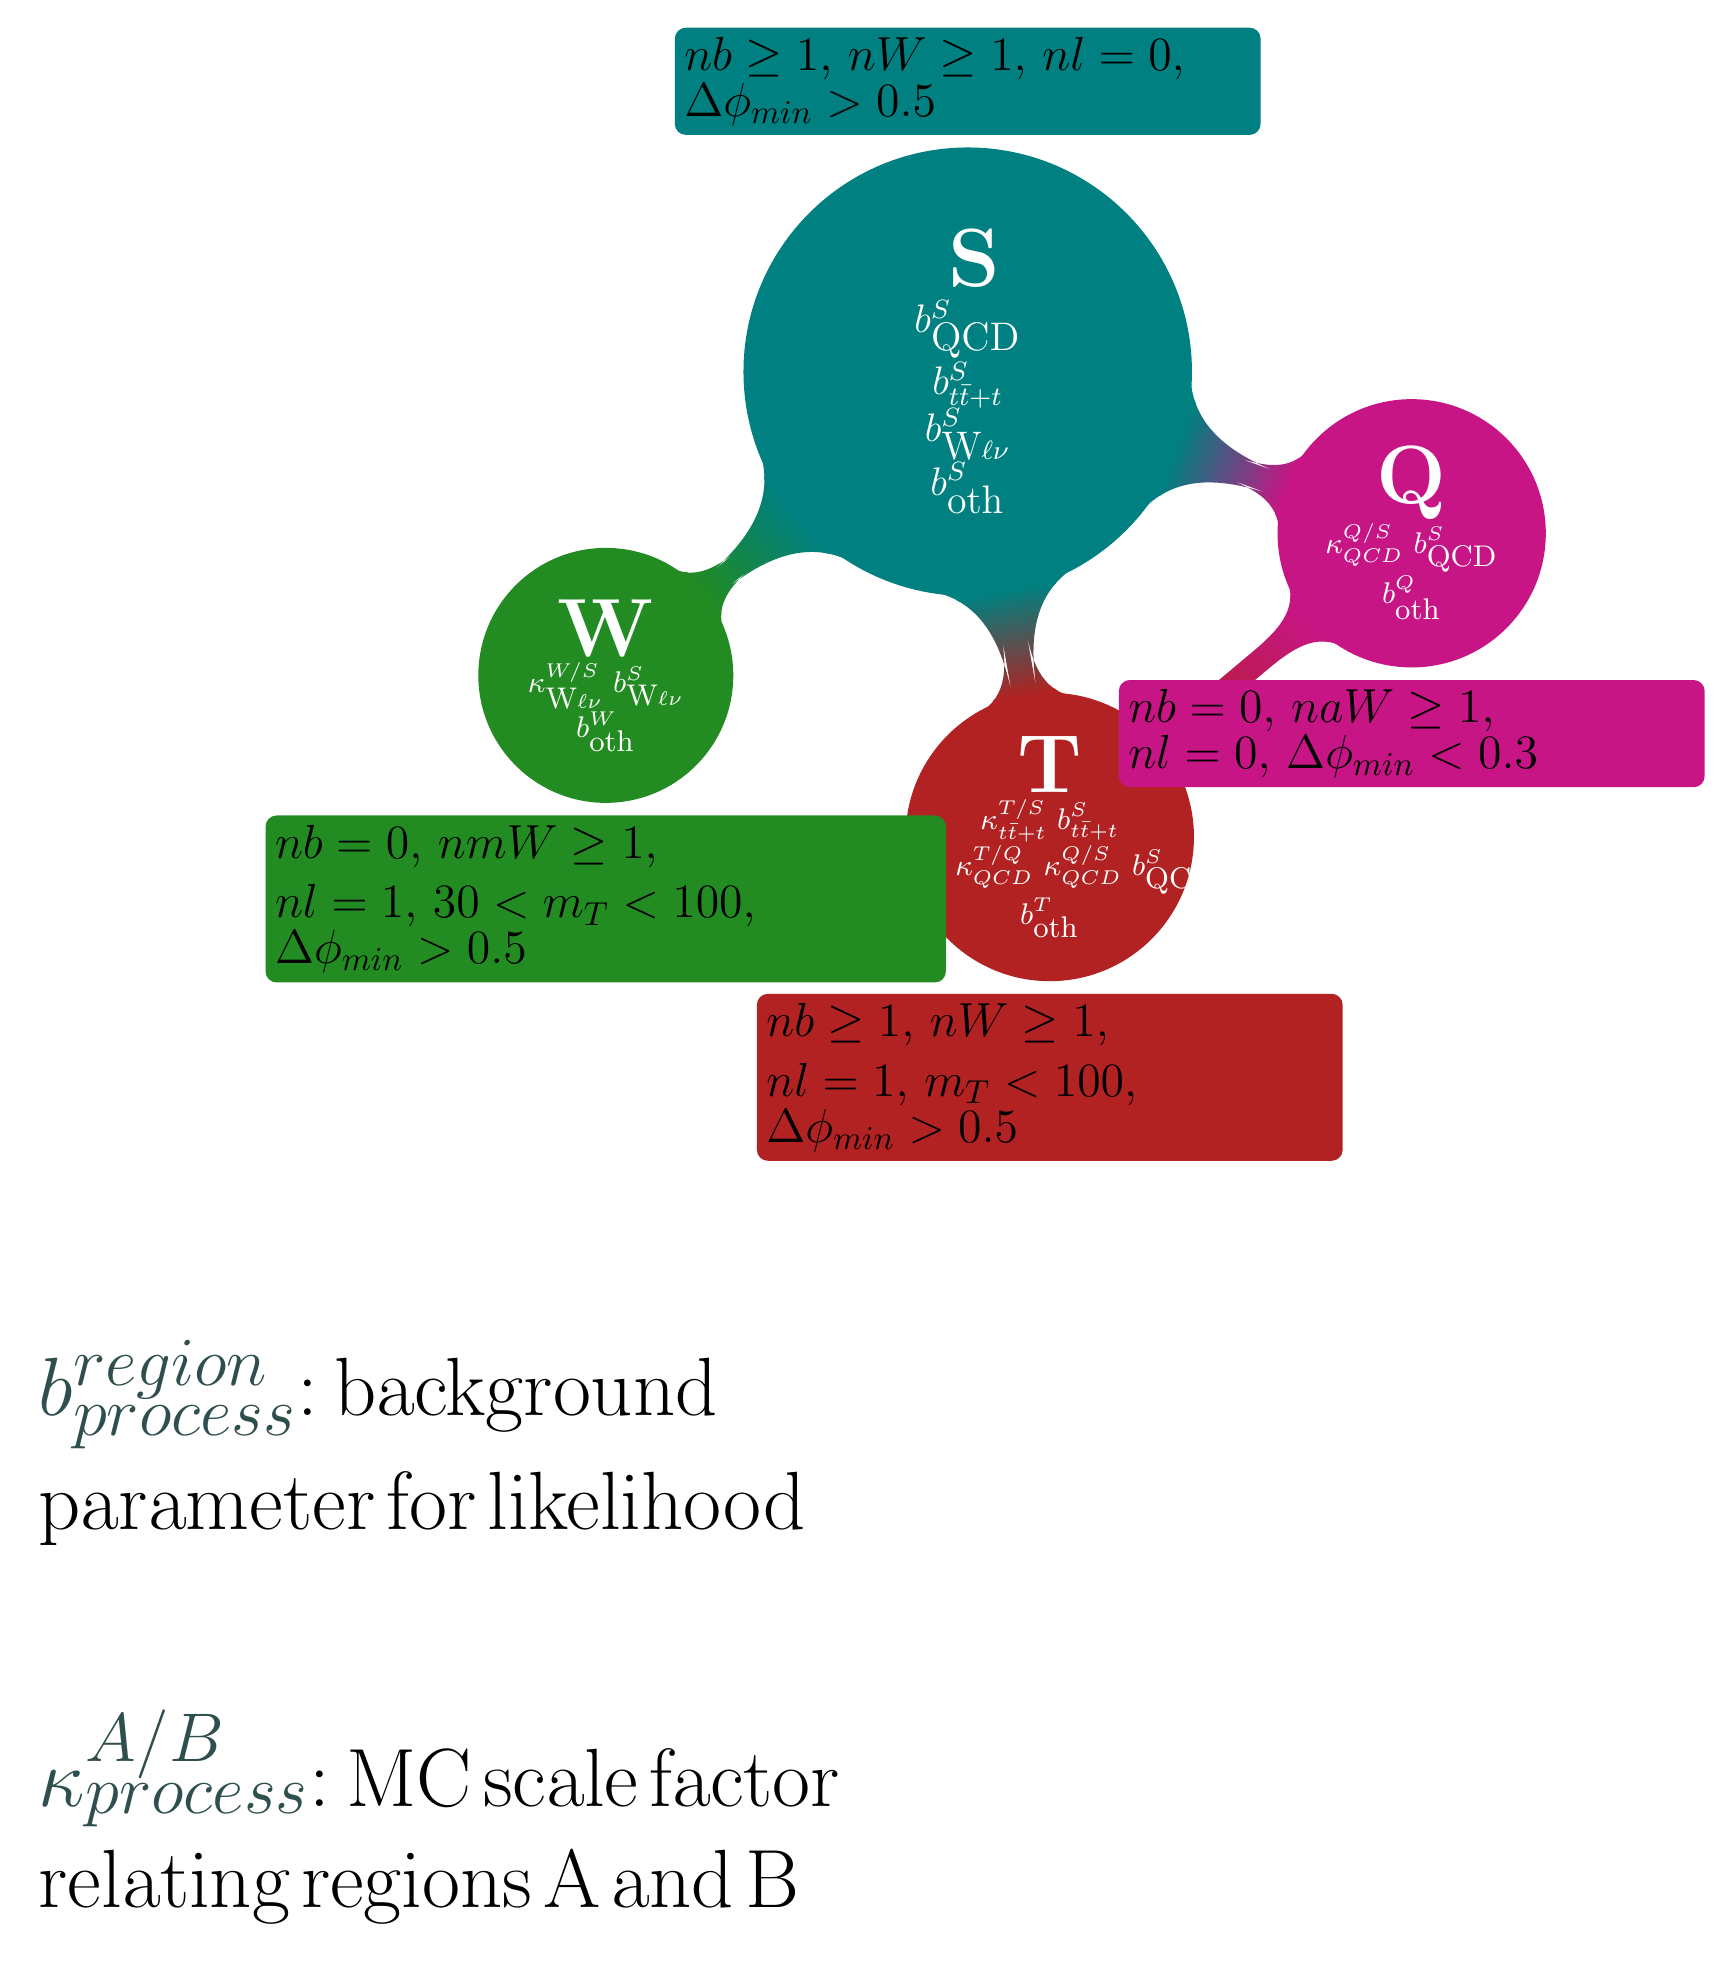
\begin{tikzpicture}[scale=1.2,transform shape]

  \path[mindmap,concept color=Teal, text=white]
    node[concept] (cS) {{\Huge \textbf{ S}} \\ $b^S_{\textrm{QCD}}$ \\$ b^S_{t\bar{t}+t}$ \\ $b^S_{\textrm{W}\ell\nu} $ \\ $b^S_{\textrm{oth}}$ }
    [clockwise from=-20]
    child[concept color=MediumVioletRed] {
      node[concept] (cQ) {{\Huge \textbf{Q}} \\ $\kappa^{Q/S}_{QCD} ~ b^S_{\textrm{QCD}}$ \\ $b^Q_{\textrm{oth}}$}
    }
    child[concept color=FireBrick] {
      node[concept] (cT) {{\Huge \textbf{T}} \\ $\kappa^{T/S}_{t\bar{t}+t} ~ b^S_{t\bar{t}+t}$\\ $\kappa^{T/Q}_{QCD} ~ \kappa^{Q/S}_{QCD} ~ b^S_{\textrm{QCD}}$  \\ $b^T_{\textrm{oth}}$ }
    }
    child[concept color=ForestGreen] { 
      node[concept] (cW) {{\Huge \textbf{W}} \\ $\kappa^{W/S}_{\textrm{W}\ell\nu} ~ b^{S}_{\textrm{W}\ell\nu}$  \\ $b^W_{\textrm{oth}}$}
    };
    %\end{scope}
    %\begin{pgfonlayer}{background}
    %  \draw[circle connection bar switch color= from (MediumVioletRed) to (FireBrick)] (cQ) edge (cT);
    %\end{pgfonlayer}
    
    \path (cQ) to[circle connection bar switch color= from (MediumVioletRed) to (FireBrick)] (cT);
    %\path (cW) to[circle connection bar switch color= from (ForestGreen) to (FireBrick)] (cT);
    
    \node [annotation,fill=Teal,above,text width=6cm] at (cS.north) {{\Large $nb\geq 1$, $nW\geq1$, $nl=0$, $\Delta\phi_{min}>0.5$}};
    \node [annotation,fill=MediumVioletRed,below,text width=6cm] at (cQ.south) {{\Large $nb=0$, $naW\geq1$,\\ $nl=0$, $\Delta\phi_{min}<0.3$}};
    %\node [annotation,fill=Goldenrod,text width=5.5cm] at (cZ) [label={[label distance=25pt]+45: {{\large $nY=0$, $nY\geq1$, $nl=2$, $60<m_{ll}<120$}}}] {};
    \node [annotation,fill=FireBrick,below ,text width=6cm] at (cT.south) {{\Large $nb\geq1$, $nW\geq1$, \\$nl=1$, $m_T<100$, \\$\Delta\phi_{min}>0.5$}};
    \node [annotation,fill=ForestGreen,below ,text width=7cm] at (cW.south) {{\Large $nb=0$, $nmW\geq1$, \\ $nl=1$, $30<m_T<100$, \\$\Delta\phi_{min}>0.5$}};

    \node[annotation,below] at (cW.south) [label={[label distance=-8cm,text width=12cm] {{\Huge \textcolor{DarkSlateGray}{$b^{region}_{process}$}: background \\[6pt] parameter for likelihood }}}] {};

    \node[annotation,below] at (cW.south) [label={[label distance=-12cm,text width=12cm] {{\Huge \textcolor{DarkSlateGray}{$\kappa_{process}^{A/B}$}: MC scale factor \\[6pt] relating regions A and B }}}] {};

\end{tikzpicture}
}
\end{center}
\end{frame}



\end{document}
